\chapter{Strategy Pattern}

\section{Định nghĩa}
Strategy Pattern là một trong những pattern thuộc nhóm hành vi (Behavior Pattern). Strategy Pattern xác định một nhóm các thuật toán, đóng gói từng cái một và khiến cho chúng có thể hoán đổi vị trí cho nhau một cách linh hoạt bên trong object. Strategy cho phép thuật toán biến đổi độc lập khi người dùng sử dụng chúng.

\section{Mục đích sử dụng}
\begin{itemize}
\item Thay đổi các thuật toán được sử dụng bên trong một đối tượng tại thời điểm run-time.
\item Khi có một đoạn mã dễ thay đổi, và muốn tách chúng ra khỏi chương trình chính để dễ dàng bảo trì.
\item Tránh sự rắc rối khi phải hiện thực một chức năng nào đó qua quá nhiều lớp con.
\item Che giấu sự phức tạp, cấu trúc bên trong của thuật toán.
\end{itemize}

\section{Strategy Pattern trong thực tế}

\section{Mô hình cấu trúc}
\begin{center}
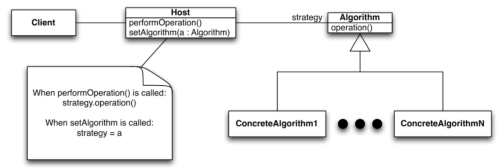
\includegraphics{GALLEYS/images/chapter9/diagram}
\end{center}
Các thành phần:
\begin{itemize}
\item Algorithm: định nghĩa các hành vi/phương thức có thể có của một Algorithm.
\item ConcreteAlgorithm : cài đặt các hành vi/phương thức cụ thể của Algorithm.
\item Host: chứa một tham chiếu đến đối tượng Algorithm và nhận các yêu cầu từ Client, các yêu cầu này sau đó được ủy quyền cho Algorithm thực hiện.
\end{itemize}
Cách tiến hành: Client (main) sử dụng Host. Algorithm được kéo ra khỏi Host. Client chỉ sử dụng giao diện công khai của Algorithm và không bị ràng buộc bởi các lớp con (concrete algorithms) cụ thể. Client có thể thay đổi hành vi của mình bằng cách chuyển đổi giữa các thuật toán cụ thể (concrete algorithms) khác nhau.
